\documentclass{article}
\usepackage[utf8]{inputenc}
\usepackage{listings}
\usepackage{graphicx}
\usepackage{float}

\setlength{\parindent}{0pt}
\lstset{
    basicstyle=\ttfamily\footnotesize,
    frame=single,
    xleftmargin=4pt,
    xrightmargin=4pt,
    breaklines=true
}

\title{Lab Report: Particle Argon Peripherals}
\author{Lue Xiong}

\begin{document}

\maketitle
\newpage

\tableofcontents
\newpage

\obeylines

\section{Introduction}
The focus of the lab is to experiment with the Google Cloud Platform to store and manipulate event data coming from the Particle Argon. Since Google Cloud Platform has a large suite of tools to use, the lab will limit the experimentation with using the following tools: Google DataStore, Google Functions, and Google Sheets. The idea here is to grasp the potential usefulness that the closed feedback loop of IoT has to offer to convenience our everyday lives.

\section{Problem Statement}
The problem to solve is to provide a solution to calculating average temperature from the last 10 temperature readings coming from the Particle Argon, using Google Cloud Platform to streamline the event data, and eventually going into Google Sheets as data in each available row. The solution should come in the form of a programming script within Google Sheets' script editor.

\section{Process}
Google Sheets has a script Integrated Development Environment (IDE) where users who are savvy enough can write their own triggers. Users are given a set of default triggers, which Google calls \textbf{Simple Triggers} but they also allow custom triggers that they call \textbf{Installable Triggers}.\\

Referenced from Figure~\ref{fig:script}, the \textbf{createSpreadsheetOnChangeTrigger()} function is executed once through the script IDE and only once. The installable trigger will be created and will stay until it is manually deleted. Subsequent invocations of this function will duplicate the installable trigger, so it is important not to do it again.\\

\begin{minipage}[c]{\textwidth}
\begin{lstlisting}
function createSpreadsheetOnChangeTrigger() {
  let spreadsheet = SpreadsheetApp.getActive()
  
  ScriptApp.newTrigger('appendAverageCalculation')
    .forSpreadsheet(spreadsheet)
    .onChange()
    .create();
}
\end{lstlisting}
\end{minipage}\ \\

The approach to solving the problem was using a few functions. The \textbf{last()} function is used to retrieve the last/latest ten temperature readings logged in Google Sheets. Once that is retrieved as a list in a list of objects, it is manipulated into the sum of all temperatures within the objects, and then divided by the amount of objects within the \textbf{calculateAverageTemperature()} function. The \textbf{appendAverageCalculation()} will lastly append the average into Google Sheets.

\begin{figure}[H]
\center
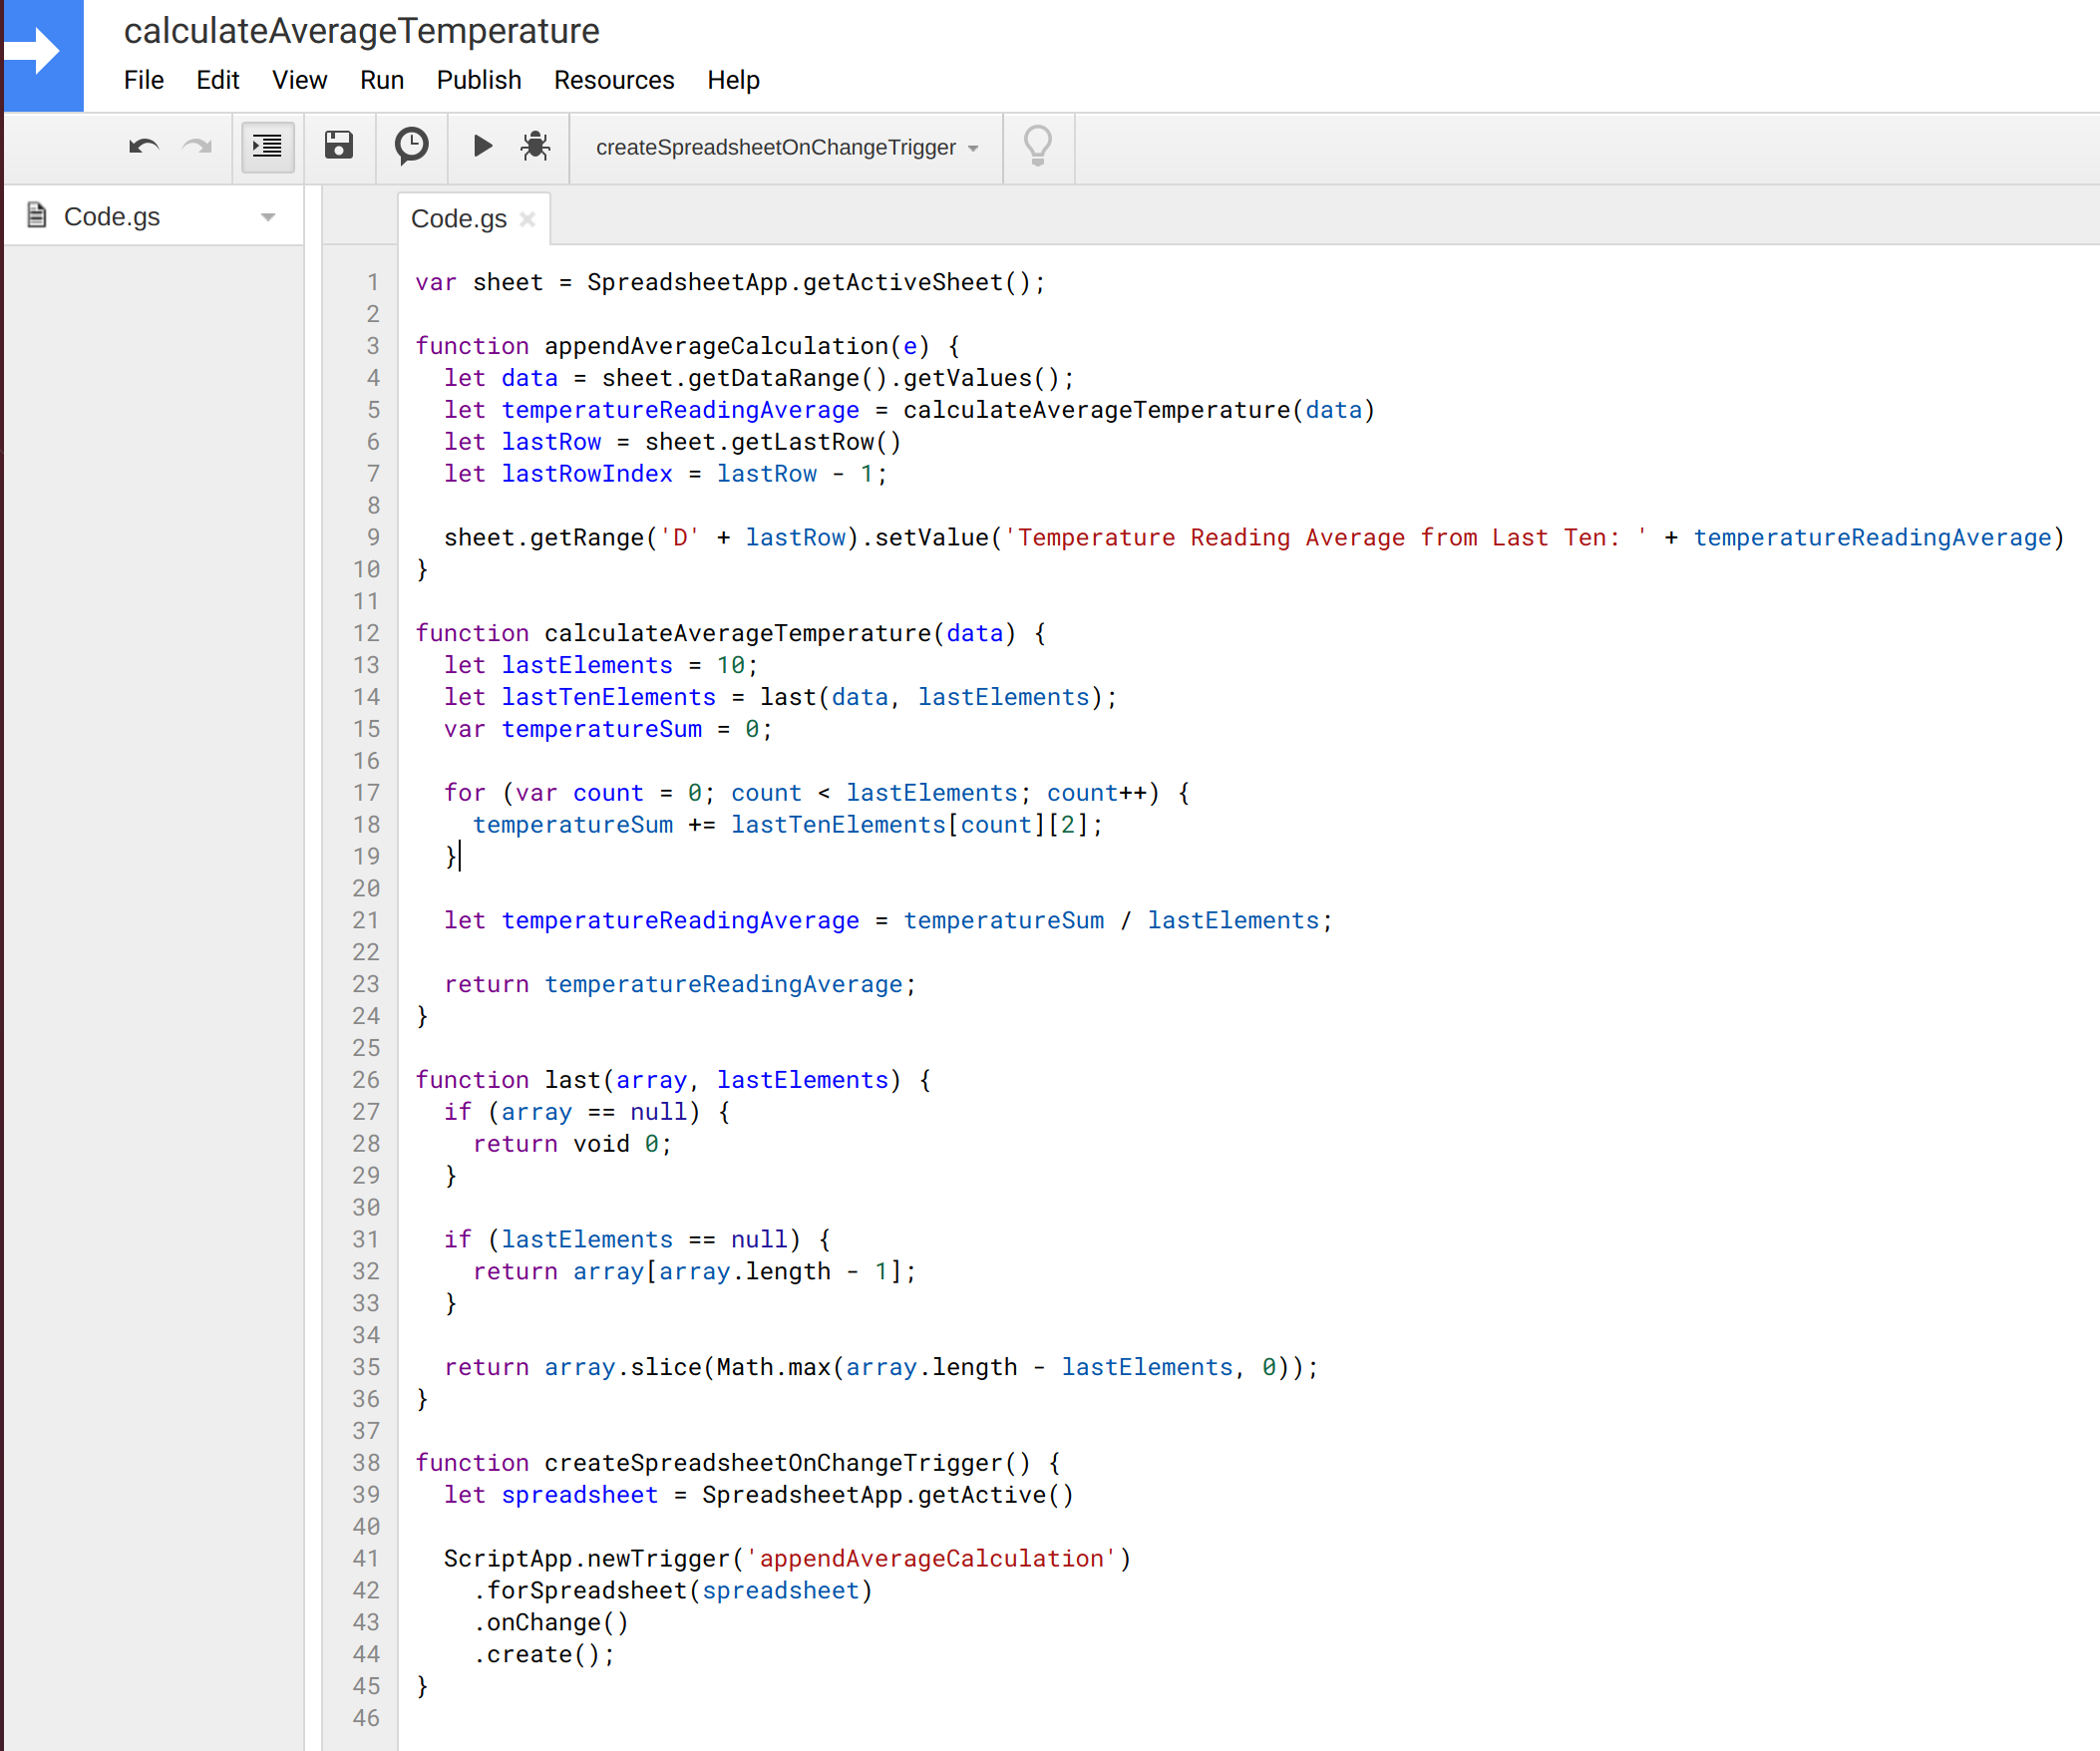
\includegraphics[width=\textwidth]{images/particle-argon-gcp-sheets-script.png}
\caption{Google Sheets Script}
\label{fig:script}
\end{figure}

Figure~\ref{fig:trigger} shows the installable trigger that is created from the function above. Figure~\ref{fig:executions} shows the executions from the trigger being called by the data event insertions into Google Sheets as shown in Figure~\ref{fig:sheets}.\\

\begin{figure}[H]
\center
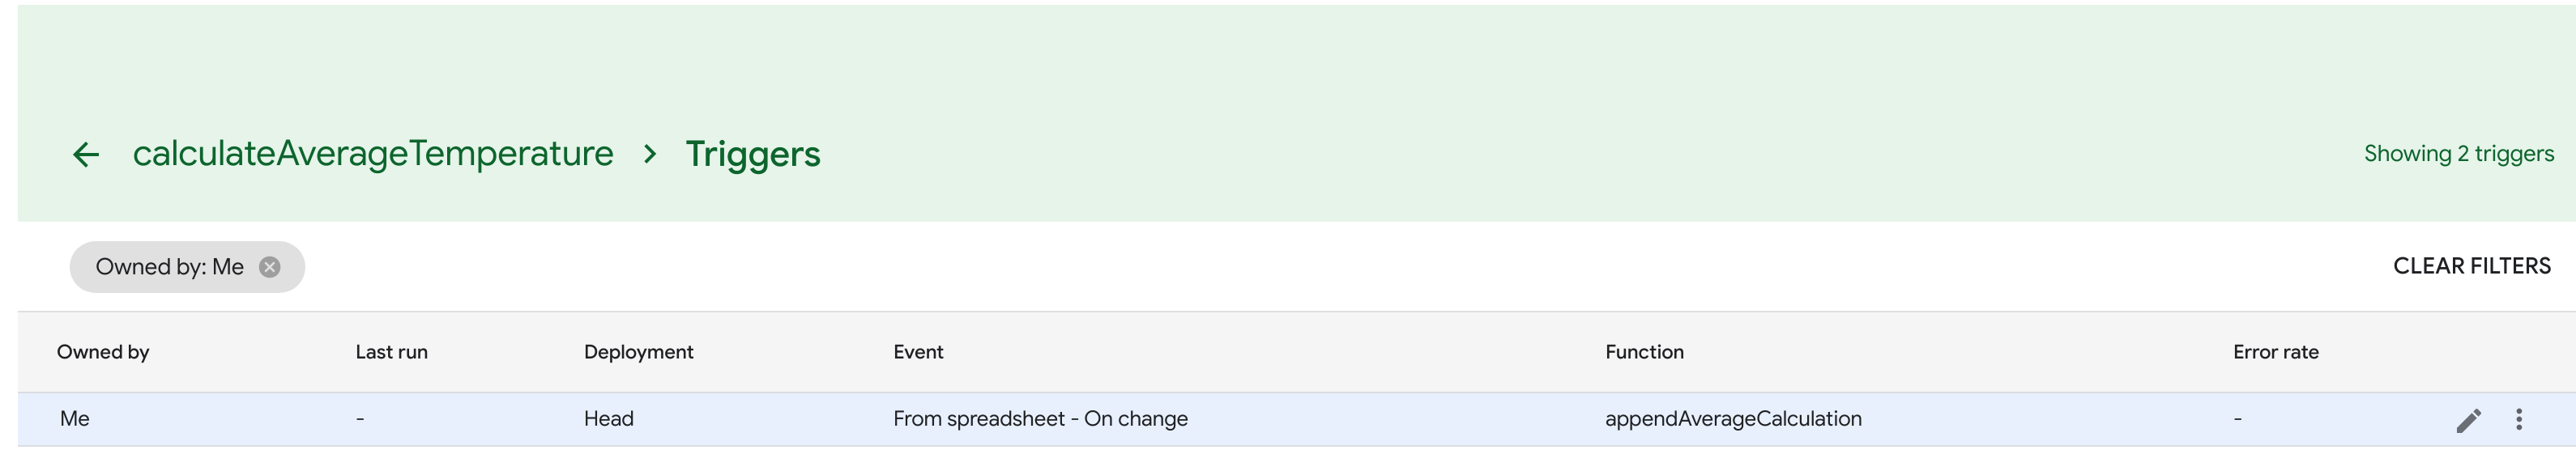
\includegraphics[width=\textwidth]{images/particle-argon-gcp-triggers.png}
\caption{Google Sheets Triggers}
\label{fig:trigger}
\end{figure}

\begin{figure}[H]
\center
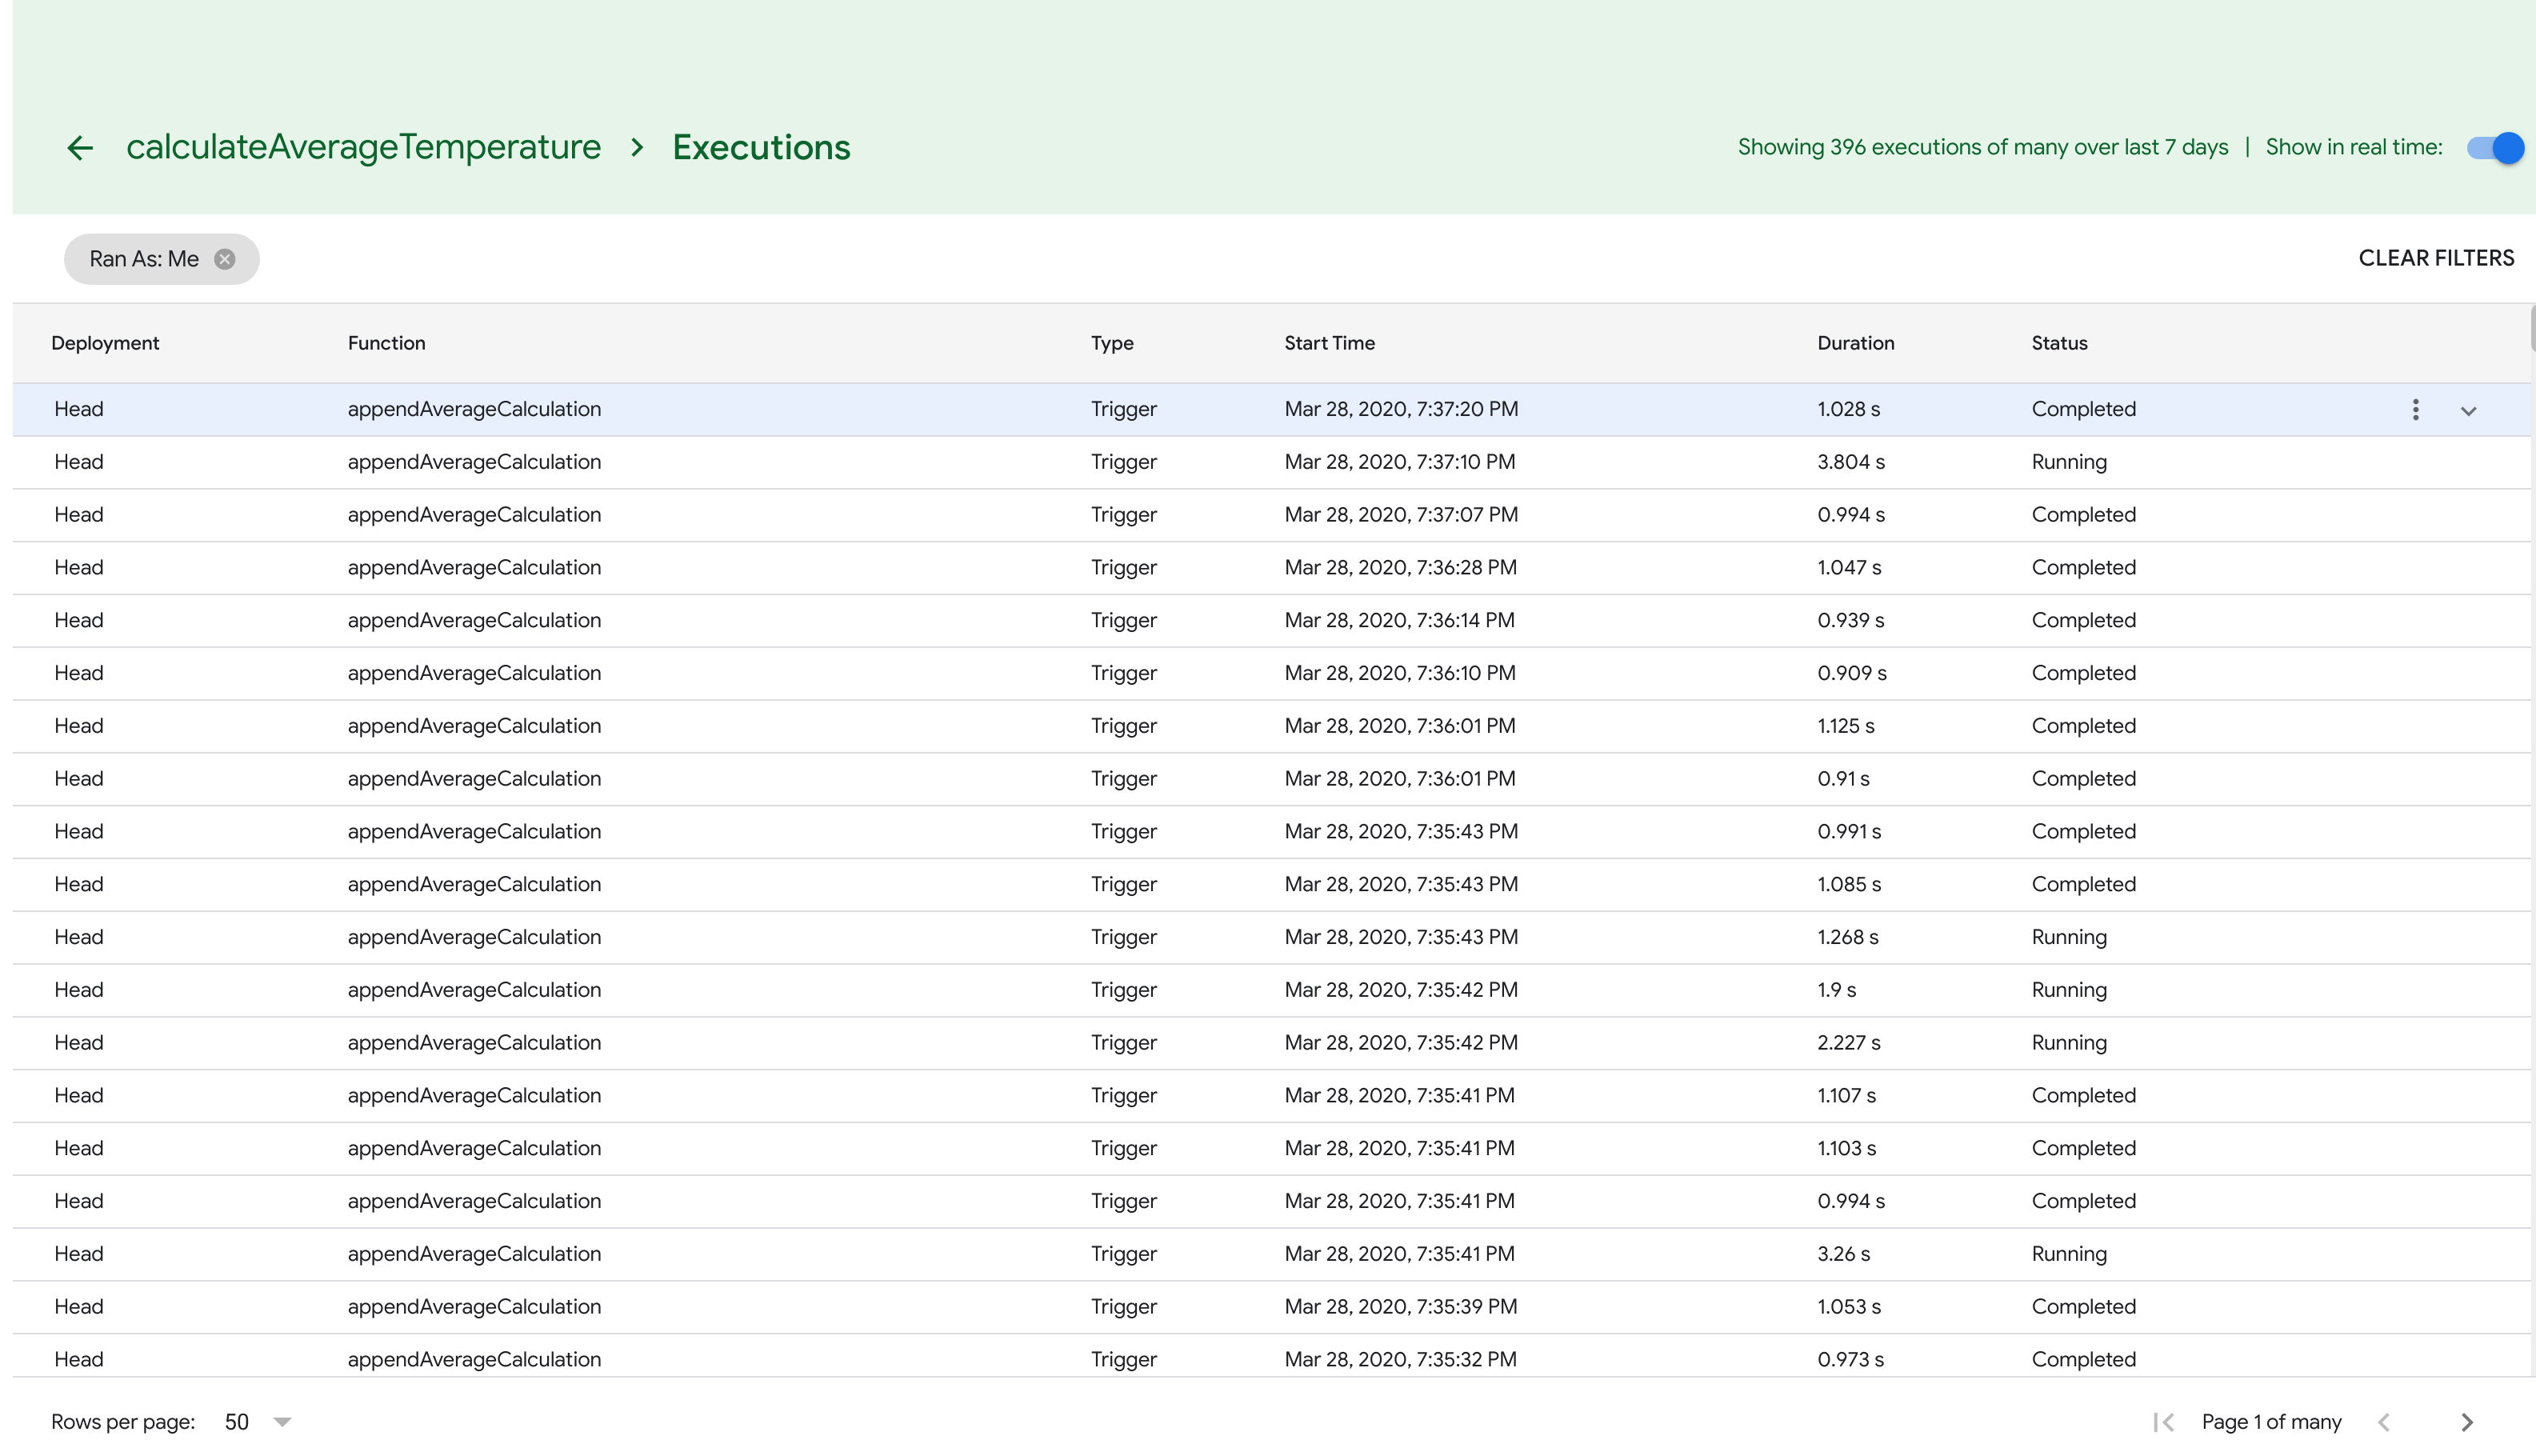
\includegraphics[width=\textwidth]{images/particle-argon-gcp-executions.png}
\caption{Google Sheets Executions}
\label{fig:executions}
\end{figure}

The important thing to point out about Figure~\ref{fig:sheets} is the intermittently missing average temperature readings. Google Sheets system has delays of when triggers are invoked versus when the trigger is able to append average temperature data from the last ten readings in each of the rows. It really is not ideal but it works nonetheless.

\begin{figure}[H]
\center
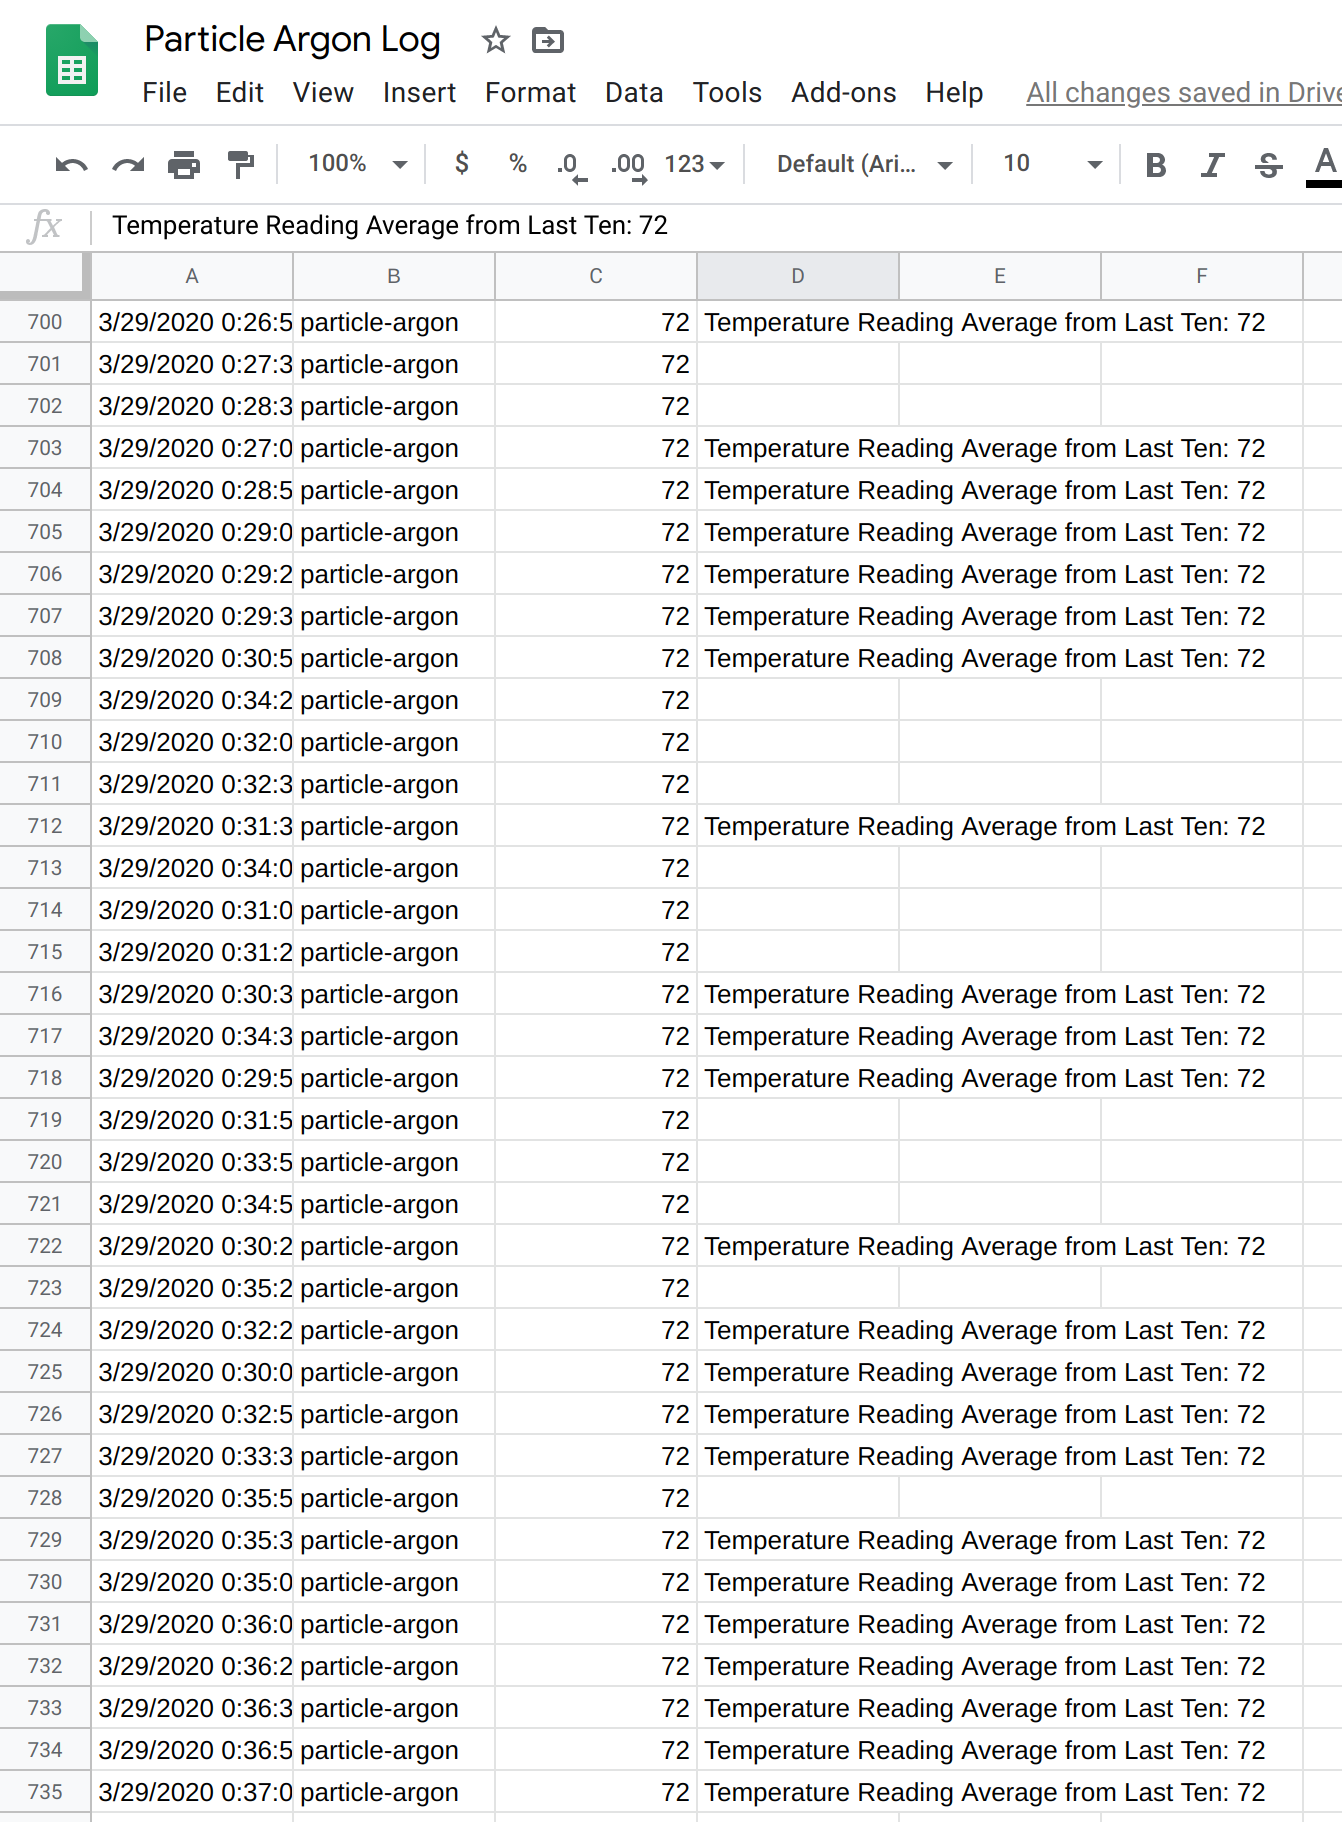
\includegraphics[width=\textwidth]{images/particle-argon-gcp-sheets.png}
\caption{Google Sheets Data}
\label{fig:sheets}
\end{figure}

\section{Discussion of Results}
The calculations were as expected, as calculating average temperature data is trivial. The difficulty of getting the desired results came from the software integration complexity. Google's API documentation is extensive, it is also overwhelming with words. Documentation can be hard to piece together unless you know key words to ironically enough, google for to get answers, scouring through results, and digging through someone else's code. Google Sheets trigger worked to calculate average temperature from the last ten readings, but it is not as robust as one would believe. It is Google afterall. Google Sheets trigger will miss triggers intermittently and has a slow trigger response before anything shows up on Google Sheets.

\section{Conclusion}
Experimenting with Google Cloud Platform shows how mature technology has grown to be able to automate tasks that typically would be manual processes. Though this technological maturity is in our presence, it does require technical expertise in terms of architecture and design, not only from a software viewpoint, but from a hardware viewpoint as well. This is truly the day-in-age in which we live that we can learn anything we want, with the assumption that we are dedicated enough to hurdle pass the steep learning curves. IoT truly is the future, in all likeliness of being used in conjunction with artificial intelligence.

\end{document}
